\documentclass{article}

\usepackage{tikz}

\begin{document}

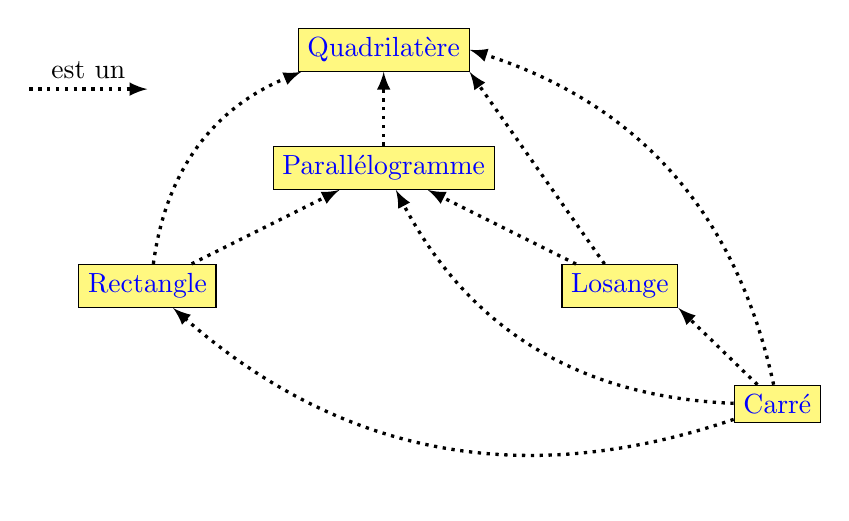
\begin{tikzpicture}
 % definition des styles
  \tikzstyle{quadri}=[rectangle,draw,fill=yellow!50,text=blue]
  \tikzstyle{estun}=[->,>=latex,very thick,dotted]
 % les neuds
  \node[quadri] (Q) at (0,3) {Quadrilat\`ere};
  \node[quadri] (P) at (0,1.5) {Parall\'elogramme};
  \node[quadri] (R) at (-3,0) {Rectangle};
  \node[quadri] (L) at (3,0) {Losange};
  \node[quadri] (C) at (5,-1.5) {Carr\'e};
 % les fleches
  \draw[estun] (P)--(Q);
  \draw[estun] (R)to[bend left](Q);  \draw[estun] (R)--(P);
  \draw[estun] (L)--(Q.south east);  \draw[estun] (L)--(P);
  \draw[estun] (C)to[bend right](Q.east); \draw[estun] (C)to[bend left](P);
  \draw[estun] (C)--(L.south east);  \draw[estun] (C)to[bend left](R);
 % la legende
  \draw[estun] (-4.5,2.5)--(-3,2.5)node[midway,above]{est un};
\end{tikzpicture}

\end{document}
